In Chapter~\ref{chapter:implementation}, we saw that an LM program operates on a graph data structure $G = (V, E)$ with nodes $V$ and edges $E$. Concurrent computation is performed non-deterministically by a set of execution threads $T$ that work on subsets of $G$.
Our implementation allows threads
to steal nodes from other threads in order to improve load balancing.  However,
there are many scheduling details that are left for our implementation to decide and which the programmer has no control over. How should a thread
schedule the computation of its sub-graph? Is node stealing beneficial to all
programs? What is the best sub-graph partitioning for a given LM program?  In order to allow custom node scheduling and partitioning, we introduce \emph{coordination facts}, a
mechanism that is indistinguishable from regular computation and that allows the
programmer to control how the runtime system executes programs. This is
an important first step in allowing the programmer to declaratively control execution. In Chapter~\ref{chapter:threads}, we further extend the language with thread-based facts to allow reasoning over the state of the execution threads.

\section{Motivation}\label{section:coord:rationale}

To motivate the need for coordination, we use the Single Source Shortest
Path~(SSSP) program, a concise program that can take advantage of custom
scheduling policies to improve its performance.
Figure~\ref{code:shortest_path_program} and Figure~\ref{code:coord:sssp_init}
show a possible implementation in LM, and Fig.~\ref{fig:shortest_path_program}
shows an instance of the program on a particular dataset. Note that in
Section~\ref{section:implementation:performance}, we presented the MSSD program
which is essentially the SSSP program modified to compute multiple shortest
distances.

The SSSP program starts with the declaration of the predicates~
(lines~\ref{line:coord:sssp_pred1}-\ref{line:coord:sssp_pred2}). As usual, the
\code{edge} predicate is a persistent predicate that describes the edges of the
graph, where the third argument is the weight of each edge. Predicate
\code{shortest} represents a valid distance and path from node \code{@1} to the
node in the first argument.  Predicate \code{relax} also represents a valid
path, and, is used to improve the distance in \code{shortest}.  The program
computes the shortest distance from node \code{@1} by improving the distance in
the \code{shortest} facts, until the shortest distance is reached in all nodes.
In Fig.~\ref{code:coord:sssp_init}, we declare an example set of initial facts
for the program: \code{edge} facts describe the graph; \code{shortest(A, +00,
[])} is the initial shortest distance (infinity) for all nodes; and
\code{relax(@1, 0, [@1])} starts the algorithm by setting the distance from
\code{@1} to \code{@1} to be 0.

\begin{figure}[ht]
\begin{LineCode}[commandchars=\*\#\&]
type edge(node, node, int).*label#line:coord:sssp_pred1&*hfill// Predicate declaration
type linear shortest(node, int, list int).
type linear relax(node, int, list int).*label#line:coord:sssp_pred2&

shortest(A, D1, P1), D1 > D2, relax(A, D2, P2)*label#line:coord:sssp_first1&*hfill// Rule 1: newly improved path
   -o shortest(A, D2, P2),
      {B, W | !edge(A, B, W) -o relax(B, D2 + W, P2 ++ [B])}.*label#line:coord:sssp_first2&

shortest(A, D1, P1), D1 <= D2, relax(A, D2, P2)*label#line:coord:sssp_second1&*hfill// Rule 2: longer path
   -o shortest(A, D1, P1).*label#line:coord:sssp_second2&
\end{LineCode}
\mycap{Single Source Shortest Path program code.}
\label{code:shortest_path_program}
\end{figure}

\begin{figure}[ht]
\begin{LineCode}[commandchars=\*\#\&]
!edge(@1, @2, 3). !edge(@1, @3, 1).
!edge(@3, @2, 1). !edge(@3, @4, 5).
!edge(@2, @4, 1).
shortest(A, +00, []).
relax(@1, 0, [@1]).
\end{LineCode}
\mycap{Initial facts for the SSSP program.}
\label{code:coord:sssp_init}
\end{figure}

\iffalse
\begin{figure}[ht]
\begin{LineCode}[commandchars=\*\#\&]
!edge(@1, @2, 3). !edge(@1, @3, 1).
!edge(@3, @2, 1). !edge(@3, @4, 5).
!edge(@2, @4, 1).
shortest(@1, 0, []).
shortest(@2, 2, [@1, @3, @2]).
shortest(@3, 1, [@1, @3]).
shortest(@4, 3, [@1, @3, @2, @4]).
\end{LineCode}
\mycap{Final database of facts for the SSSP program.}
\label{code:coord:sssp_end}
\end{figure}
\fi
\begin{figure}
\begin{center}
   \begin{subfigure}[b]{0.49\textwidth}
      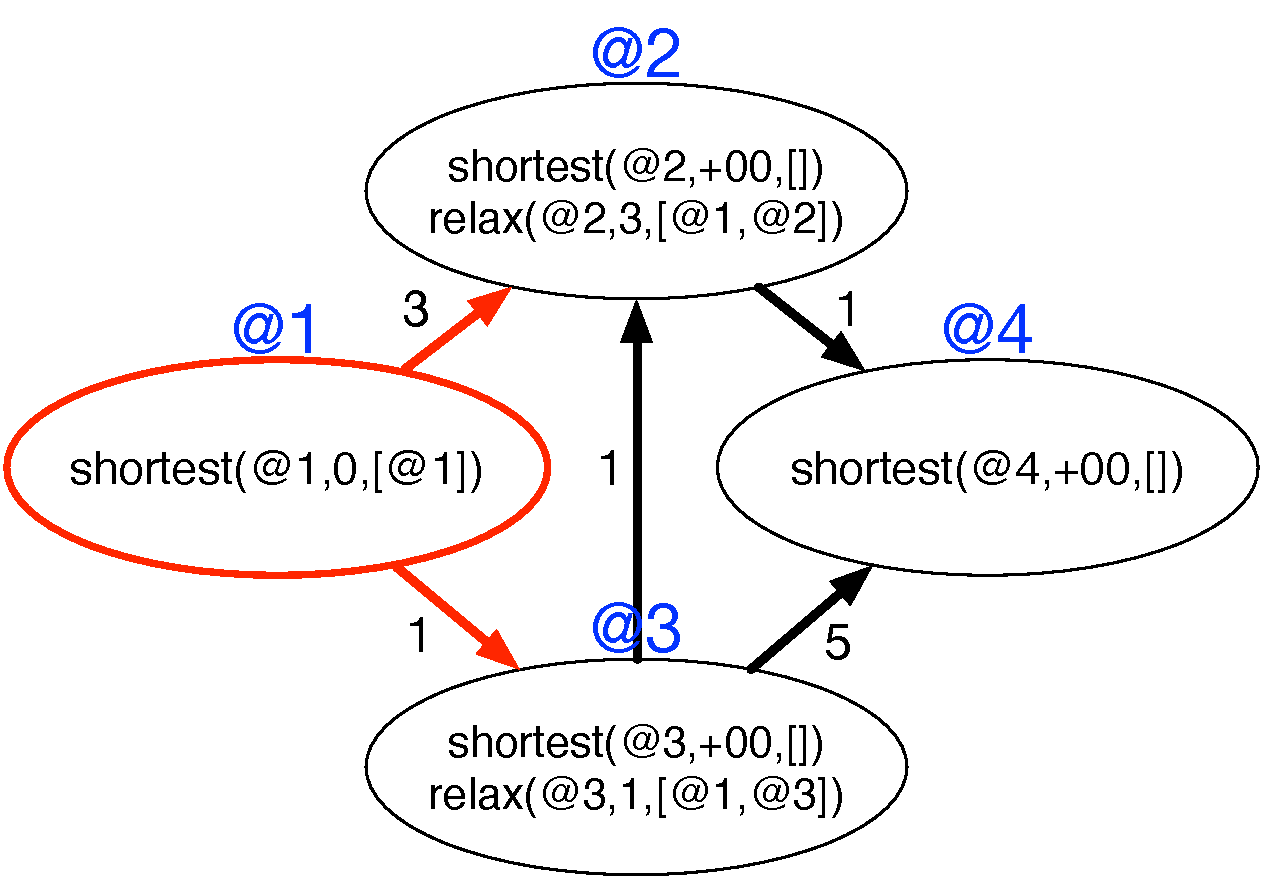
\includegraphics[width=\textwidth]{figures/sssp/shortest2}
      \mycap{}
   \end{subfigure}
   \begin{subfigure}[b]{0.49\textwidth}
      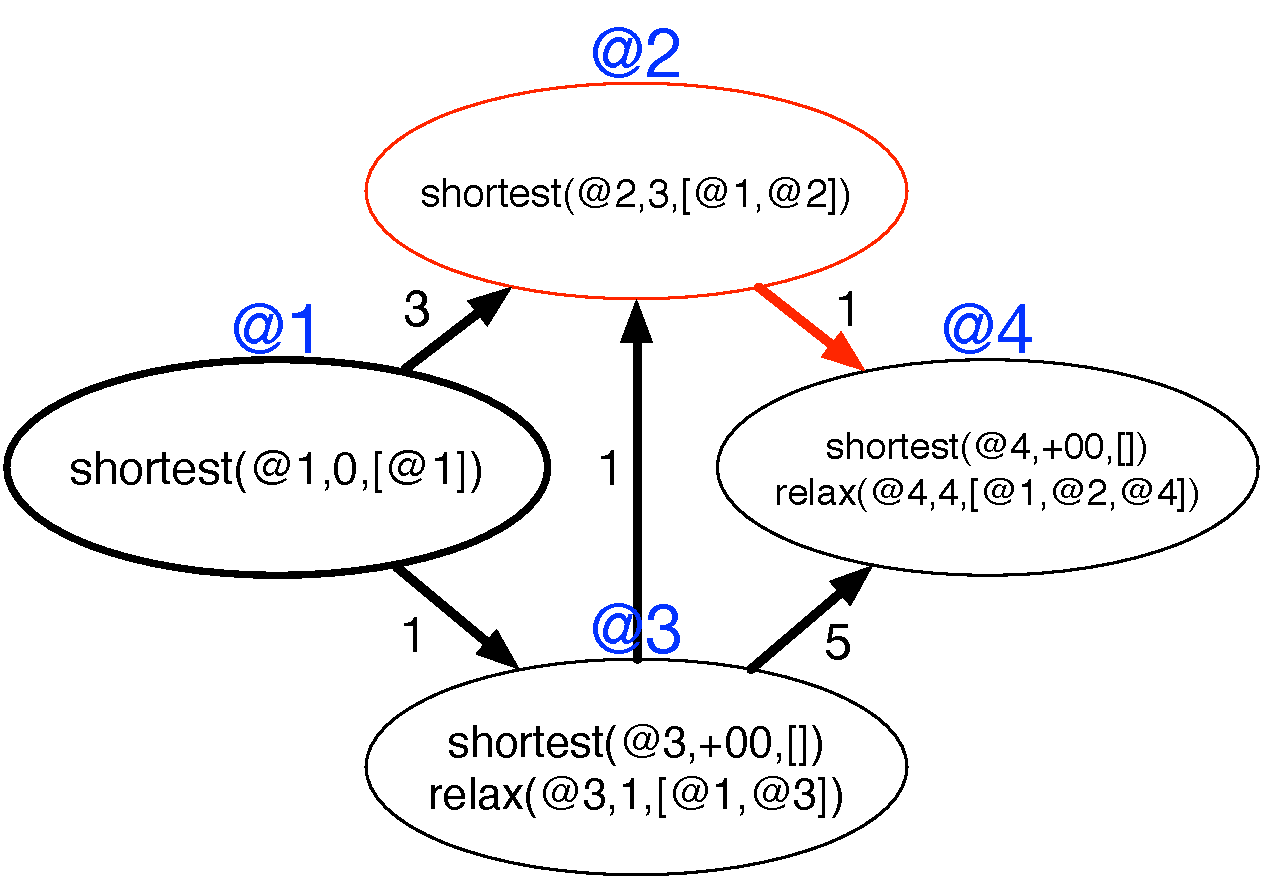
\includegraphics[width=\textwidth]{figures/sssp/shortest3}
      \mycap{}
   \end{subfigure}
   \begin{subfigure}[b]{0.49\textwidth}
      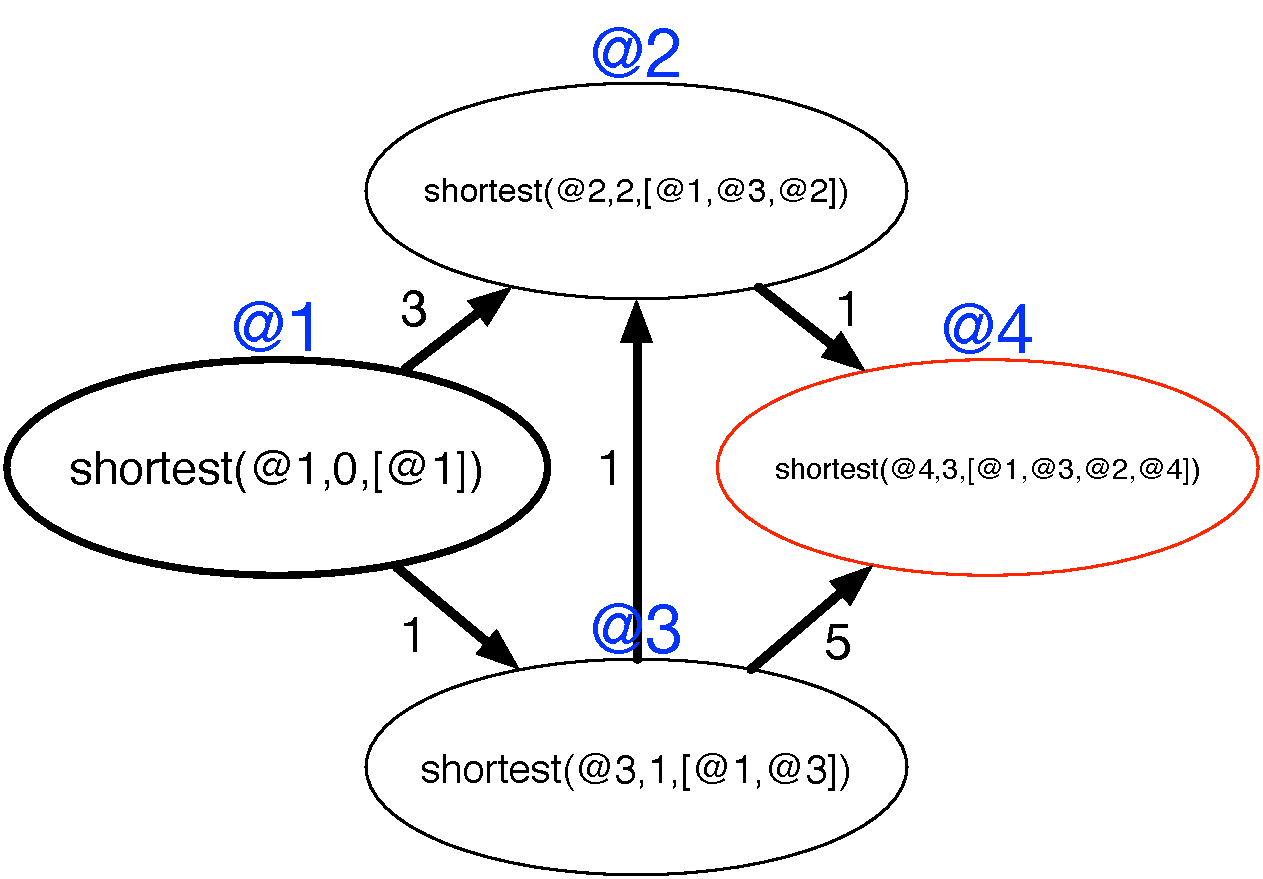
\includegraphics[width=\textwidth]{figures/sssp/shortest8}
      \mycap{}
   \end{subfigure}
\end{center}

\mycap{Graphical representation of an example dataset for the SSSP program: (a) represents the
   program's state after propagating the initial distance at node \code{@1}, followed by (b)
   where the first rule is applied in node \code{@2}, and (c) represents the
   final state of the program, where all the shortest paths have been computed.}

\label{fig:shortest_path_program}
\end{figure}

The first rule of the program
(lines~\ref{line:coord:sssp_first1}-\ref{line:coord:sssp_first2}) reads as
follows: if the current \code{shortest} path \code{P1} with distance \code{D1}
is larger than a new path \code{relax} with distance \code{D2}, then replace the
current shortest path with \code{D2}, delete the new \code{relax} path and
propagate new paths to the neighbors (comprehension at
line~\ref{line:coord:sssp_first2}). The comprehension iterates over the edges of
node \code{A} and derives a new \code{relax} fact for each node \code{B} with
the distance \code{D2 + W}, where \code{W} is the weight of the edge. For
example, in Fig.~\ref{fig:shortest_path_program}(a) we apply rule 1 in node
\code{@1} and two new \code{relax} facts are derived at node \code{@2} and
\code{@3}.  Fig.~\ref{fig:shortest_path_program}(b) is the result after
applying the same rule but at node \code{@2}.

The second rule of the program
(lines~\ref{line:coord:sssp_second1}-\ref{line:coord:sssp_second2}) retracts a
\code{relax} fact that has a longer distance than the current shortest distance
stored in \code{shortest}. There are many opportunities for custom scheduling
in the SSSP program. For instance, after applying rule 1 in
Fig.~\ref{fig:shortest_path_program}(a), it is possible to either apply rules
in either node \code{@2} or node \code{@3}.  This decision depends largely on
implementation factors such as node partitioning and number of threads in the
system. Still, it is easy to prove that, independent of the particular scheduling used, the final
result presented in Fig.~\ref{fig:shortest_path_program}(c) is always achieved.

The SSSP program is concise and declarative but its performance depends on the
order in which nodes are executed. If nodes with greater distances are
prioritized over other nodes, the program will generate more \code{relax} facts
and it will take longer to reach the shortest distances. From
Fig.~\ref{fig:shortest_path_program}, it is clear that the best scheduling is
the following: \code{@1}, \code{@3}, \code{@2} and then \code{@4}, where only 4
\code{relax} facts are generated. If we had decided to process nodes in order
\code{@1}, \code{@2}, \code{@4}, \code{@3}, \code{@4}, \code{@2}, then 6
\code{relax} facts would have been generated.  The optimal solution for SSSP is
to schedule the node with the shortest distance, which is essentially the
Dijkstra shortest path algorithm~\cite{Dijkstra}. Note how it is possible to
change the complexity of the algorithm by simply changing the order of node
computation, but still retain the same declarative nature of the program.



\section{Types of Facts}

LM introduces the concept of coordination that allows the programmer to write
code that changes how the runtime system schedules and partitions the set of
available nodes across the threads of execution. Beyond the distinction between
linear and persistent facts, LM further classifies facts into 3 categories:
\emph{computation facts}, \emph{structural facts} and \emph{coordination facts}.
Predicates are also classified accordingly.

Computation facts are regular facts used to represent the program state. In
Fig.~\ref{code:shortest_path_program}, \texttt{relax} and \texttt{shortest} are
both computation facts.

Structural facts describe information about the connections between the nodes in
the graph. In Fig.~\ref{code:shortest_path_program}, \texttt{edge} facts are
structural since the corresponding \texttt{edge} is used for communication
between nodes.  Note that structural facts can also be seen as computation facts
since they are heavily used in the program's logic.

\emph{Coordination facts} are classified into \emph{scheduling facts} and
\emph{partitioning facts} and allow the programmer to change how the runtime
schedules nodes and how it partitions the nodes among threads of execution,
respectively. Coordination facts can be used either in the LHS, RHS or both.
This allows scheduling and partition decisions to be made based on the state of
the program and on the state of the underlying machine.  In this fashion, we
keep the language declarative because we reason logically about the state of
execution, without the need to introduce extra-logical operators into the
language that would generate significant issues when proving properties about
the programs.

Both scheduling and partitioning facts can be further classified into two kinds
of facts: \emph{sensing facts} and \emph{action facts}. Sensing facts are used
to sense information about the underlying runtime system, such as the placement
of nodes in the CPU and scheduling information.\footnote{In the original
   Meld~\cite{ashley-rollman-iclp09}, sensing facts were used to get information
about the outside world, like temperature, touch data, neighborhood status,
etc.}

Action facts are used to apply coordination operations on the runtime system.
Action facts are linear facts which are consumed when the corresponding action
is performed.\footnote{Like sensing facts, action facts were also introduced in the
original Meld and were used to make the robots perform actions in the outside
world (e.g., moving, changing speed).} We use them to change the order in
which nodes are evaluated in the runtime system and to make partitioning
decisions (assign nodes to threads). It is possible to give hints to the virtual
machine in order to prioritize the computation of some nodes.

With sensing and action facts, we can write \emph{meta-rules} that will
sense the state of the runtime system and then apply decisions in order to
improve execution speed or change partitioning information. In most situations,
this set of rules can be added to the program without modifying the meaning of
the original rules.


\section{Scheduling Facts}\label{sec:coord:fifo}


In order to allow different scheduling strategies, we introduce the concept of
\emph{node priority} by assigning a priority value to every node in the program
and by introducing coordination facts that manipulate such priority values.  By
default, nodes have no priority and can be picked in any order. In our
implementation, we use a FIFO approach because older nodes tend to have a higher
number of unexamined facts, from which to derive subsequent new facts.

We have two kinds of priorities: a \emph{temporary priority} and a \emph{default
   priority}. A temporary priority momentarily changes the default priority $D$
of a node, so that once the node is done, the priority will default back to $D$.
Initially, all nodes have a default priority of $-\infty$.

The following list presents the action facts available to manipulate the
scheduling decisions of the system:

\begin{itemize}
   \item \code{set-priority(node A, float F)}: This sets the
   temporary priority of \texttt{A} to \texttt{F}. If \texttt{A} has priority
   \texttt{F'}, we only change the priority if \texttt{F} is higher. The programmer
   can decide if priorities are to be ordered in ascending or descending order.
   \item \code{add-priority(node A, float F)}: Increases,
   temporarily, the priority of node \texttt{A} by \texttt{F}.
   \item \code{remove-priority(node A)}: Removes the temporary priority from node
   \texttt{A}.
   \item \code{schedule-next(node A)}: Changes the temporary priority of node
   \texttt{A} to be $+\infty$.
   \item \code{set-default-priority(node, float)}: Sets the default
   priority of the node.
   \item \code{stop-program()}: Immediately stops the execution of the whole program.
\end{itemize}

LM provides the sensing facts \code{priority(node A, float P)} and
\code{default-priority(node A, float DP)} in order to provide the priority
\code{P} or the default priority \code{DP} of node \code{A}, respectively.
Sensing facts can only be used in the body of rules and are exempt from the
constraint that forces every fact used in the body to have the same first
argument. Also note that when sensing facts are used to prove new facts, they
are re-derived automatically. All the coordination facts are linear and are
consumed when used in the body of a rule.  The system creates the necessary code
to re-derive them without programmer interaction. Likewise,
\texttt{set-priority} and \texttt{set-default-priority} update the value of
\texttt{priority} facts by retracting and re-asserting them but this is done
automatically by the runtime system.

The priorities assigned to nodes are respected on a thread basis, therefore a
thread will always pick the highest priority node on its sub-graph but not the
highest priority node of the whole graph.
Figure~\ref{fig:coordination:priorities} shows a graph that is being processed
by two threads \texttt{T0} and \texttt{T1}. The order for \texttt{T0} will be
\texttt{@0}, \texttt{1}, \texttt{@3}, \texttt{@2} and for thread \texttt{T1} it
will be \texttt{@4}, \texttt{@6}, \texttt{@5}.  Priorities can also be seen as
hints because they do not provide a global ordering but only a local ordering
that is somewhat similar to the global ordering. The only exception is
\texttt{schedule-next}, which, when the target node is located in the current
thread, will always be enforced.

Note that priorities of nodes can be set from any node in the graph, even if those nodes
live on different threads. Of course, this implies communication between
threads.

\begin{figure}
\begin{center}
   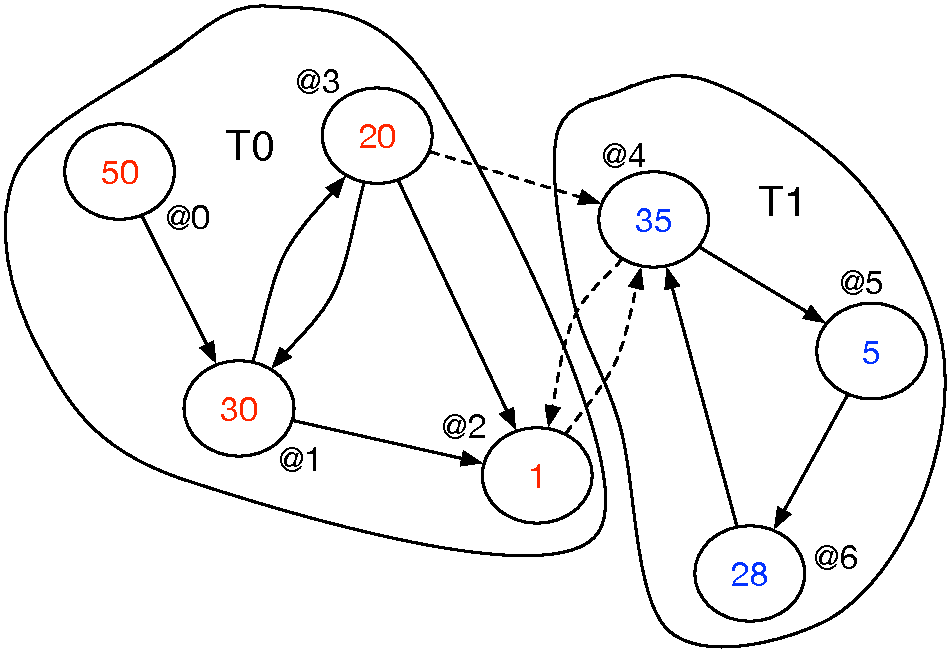
\includegraphics[width=0.7\textwidth]{figures/coordination/priorities.pdf}
\end{center}
\caption{Priorities with sub-graph partitioning. Priorities are used on a
   per-thread basis therefore thread \texttt{T0} schedules \texttt{@0} to
   execute, while \texttt{T1} schedules node \texttt{@4}.}
\label{fig:coordination:priorities}
\end{figure}


\section{Partitioning Facts}
We provide several coordination facts for dealing with node partitioning among
the running threads. Since each node is placed in some thread, the partitioning
facts revolve around thread placement.  In terms of action facts, we have the
following:

\begin{itemize}
   \item \code{set-thread(node A, thread T)}: Moves node \texttt{A} to thread
   \texttt{T}.

   \item \code{set-affinity(node A, node B)}: Places node \texttt{B} in
   the thread of node \texttt{A}.

   \item \code{set-static(node A)}: Forces node \texttt{A} to stay in the
   same thread indefinitely.

   \item \code{set-moving(node A)}: Allows node \texttt{A} to move freely
   between threads.

\end{itemize}

As an example of \texttt{set-thread}, consider again the graph in
Fig.~\ref{fig:coordination:priorities}. If a coordination fact
\texttt{set-thread(@2, T1)} is derived, then node \texttt{@2} will become part
of the sub-graph of thread \texttt{T1}. The result is shown in
Fig.~\ref{fig:coordination:partitioning}.

\begin{figure}
\begin{center}
   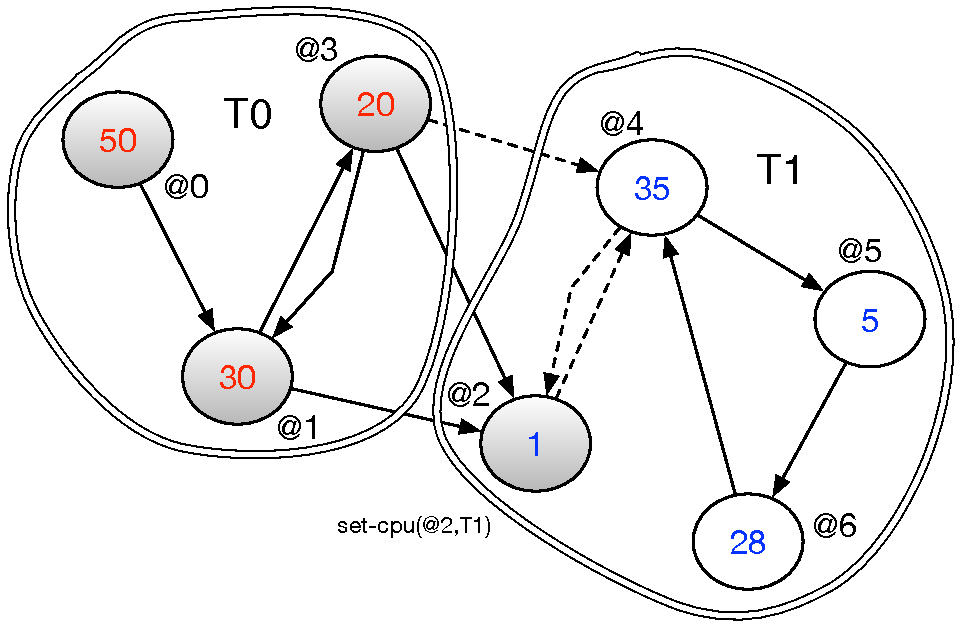
\includegraphics[width=0.6\textwidth]{figures/coordination/partitioning.pdf}
\end{center}
\caption{Moving node \texttt{@2} to thread \texttt{T1} using
   \texttt{set-thread(@2, T1)}.}
\label{fig:coordination:partitioning}
\end{figure}

Sensing facts retrieve information about node placement and are specified as
follows:

\begin{itemize}

   \item \code{thread-id(node A, thread T)}: Linear fact that maps node \code{A}
      to thread \code{T} which \code{A} belongs to. Fact \code{set-thread}
      implicitly updates fact \code{thread-id}.

   \item \code{is-static(node A)}: Fact available at node \texttt{A} if
   \item \code{is-moving(node A)}: Fact available at node \texttt{A} if
      \texttt{A} is allowed to move between threads.

      \texttt{A} is not allowed to move between threads.

   \item \code{just-moved(node A)}: Linear fact derived by the
      \code{set-thread} action if, at that moment, the node \code{A} is running
      on the target thread.

\end{itemize}



\section{Global Directives}\label{sec:coordination:global}

We also provide a few global coordination statements that cannot be specified
as sensing or action facts but are still important:


\begin{itemize}

   \item \texttt{priority @order ORDER} (\texttt{ORDER} can be either \code{asc}
      or \code{desc}): Defines if priorities are to be selected by the smallest
      or the greatest value, respectively.

   \item \texttt{priority @default P}: Informs the runtime system that all nodes
      must start with default priority \code{P}. Alternatively, the programmer can define a
      \texttt{set-default-priority(A, P)} fact.

   \item \texttt{priority @base P}: Informs the runtime system that the
      \emph{base priority} should be \code{P}. The base priority is, by default,
      0 when the priority ordering is \code{desc} and $+\infty$ when the ordering
      is \code{asc} and represents the smallest priority value possible.

   \item \texttt{priority @initial P}: Informs the runtime system that all nodes
   must start with temporary priority \code{P}. Alternatively, the programmer can define an
      \texttt{set-priority(A, P)} fact. The default is value is the one defined
      as the \emph{base priority}.

\end{itemize}


\section{Implementation}
In order to support priorities and node partitioning, we extended the work queue
of each thread, as presented in Fig.~\ref{fig:implementation:vm_overview}, to
include two new pairs of queues: two doubly linked lists known as the
\emph{standard queue} and two min/max heaps known as the \emph{priority queue}.
The standard queue contains nodes without priorities and supports push into
tail, remove node from the head, remove arbitrary node, and remove first half of
nodes.  The priority queue contains nodes with priorities and is implemented as
a binary heap array.  It supports the following operations: push into the heap,
remove the \emph{min} node, remove an arbitrary node, remove half of the nodes
(vertical split), and priority update.  Operations for removing half of the
queue are implemented in order to support node stealing, while operations to
remove arbitrary nodes or update priority allows threads to change the priority
of nodes.  Table~\ref{fig:implementation:table_queue} shows the complexity of
queue operations and compares the standard queue against the priority queue.
Except for the remove half operation, priority queue operations are more
expensive.

\begin{table}[h]
   \begin{tabular}{| c | c | c |}
      \hline
      \textbf{Operation} & \textbf{Standard queue} & \textbf{Priority Queue} \\
      \hline
      Push & $\mathcal{O}(1)$ & $\mathcal{O}(\log{N})$ \\ \hline
      Pop & $\mathcal{O}(1)$ & $\mathcal{O}(\log{N})$ \\ \hline
      Remove & $\mathcal{O}(1)$ & $\mathcal{O}(\log{N})$ \\ \hline
      Remove Half & $\mathcal{O}(N)$ & $\mathcal{O}(\log{N})$ \\ \hline
      Priority Update & - & $\mathcal{O}(\log{N})$ \\ \hline
   \end{tabular}
   \caption{Complexity of queue operations for both the standard
      queue and the priority queue.}
   \label{fig:implementation:table_queue}
\end{table}

\begin{figure*}[t]
\centering
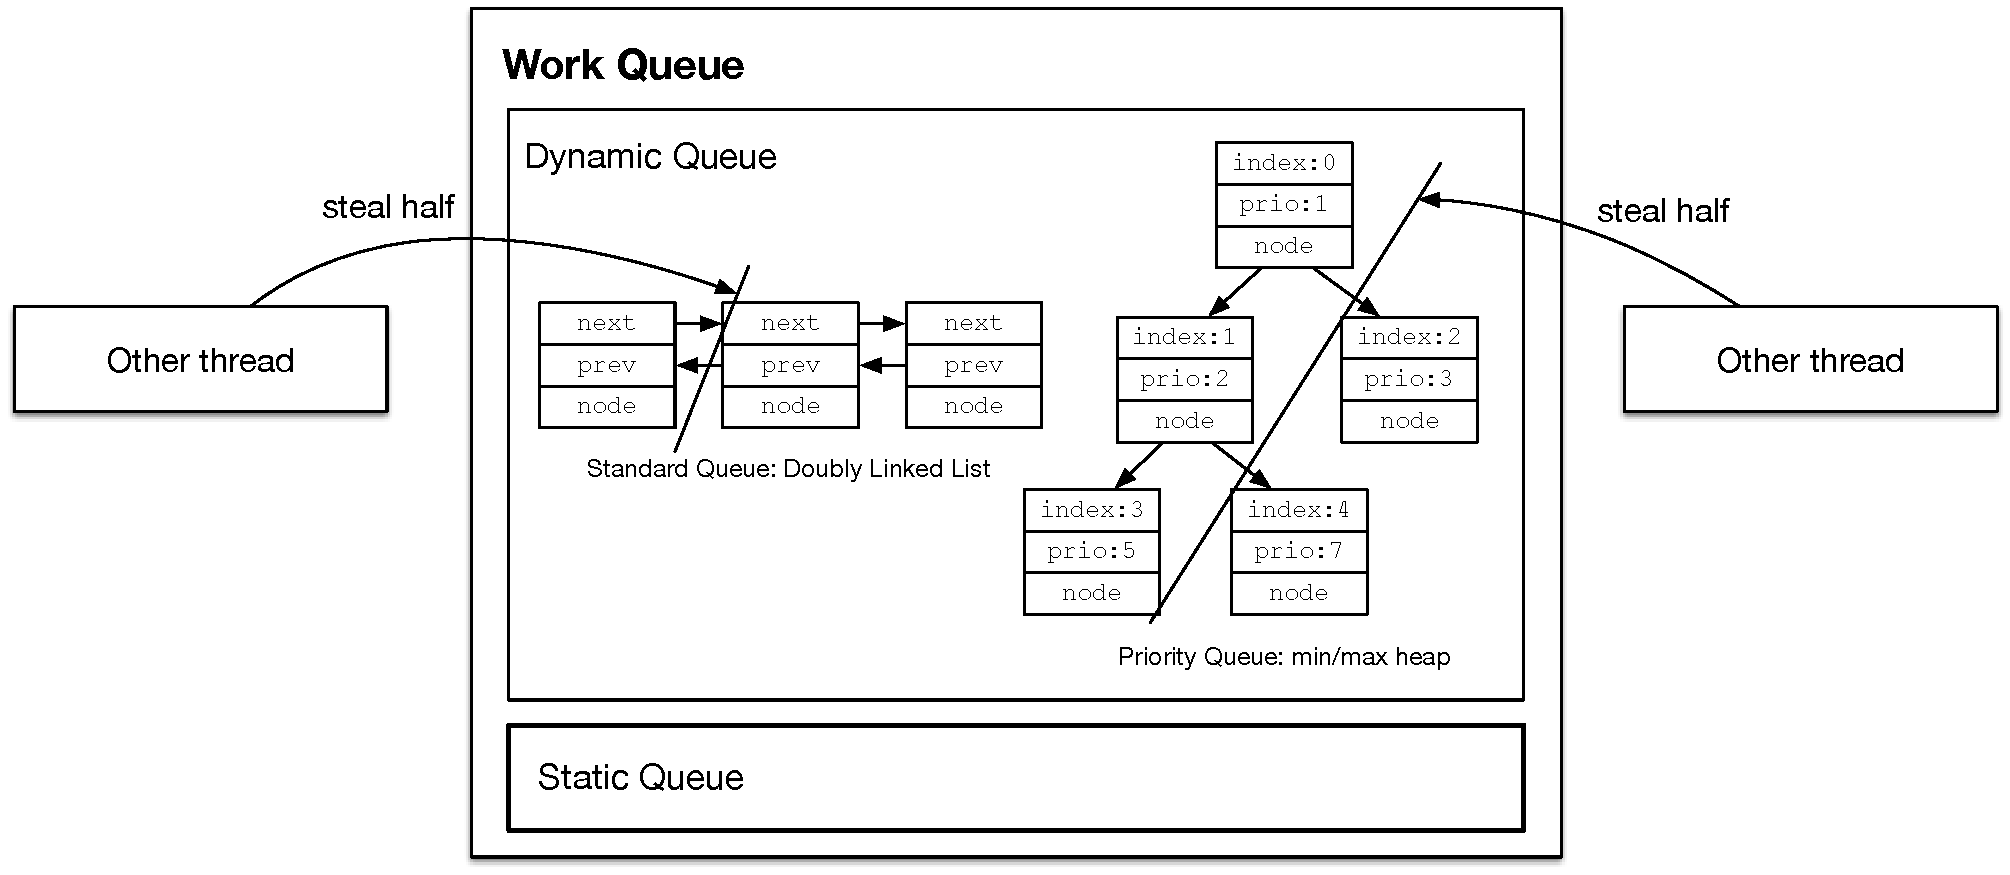
\includegraphics[width=0.95\textwidth]{figures/implementation/work_queue.pdf}
\caption{Thread's work queue and its interaction with other threads: the dynamic queue contains nodes that can be
   stolen while the static queue contains nodes that cannot be stolen. Both
   queues are implemented with one standard queue and one priority queue.}
\label{fig:implementation:work_queue}
\end{figure*}

The \texttt{next} and \texttt{prev} pointers of the standard queue are part of
the node structure in order to save space. These pointers are also used in the
priority queue but for storing the current priority and the index in the binary
heap array. Both the standard and priority queue are implemented as a pair of
queues. This first queue of each pair is a \emph{static queue} which contains
nodes that cannot be stolen and the second queue is the \emph{dynamic queue}
which contains nodes which can be stolen by other threads.
Figure~\ref{fig:implementation:work_queue} presents an overview of the two pairs
of queues and how the remove half operations are implemented in both queues in
order to support node stealing.  In the regular queue, the first $n/2$ elements
are removed from the front of the list and, in the priority queue, the binary
heap is split vertically for improved distribution of priorities.

Remember that to minimize inter-thread communication, node priorities are
implemented at the thread level, i.e., when a thread picks the highest priority
node from the priority queue, it picks the highest priority node from its
subgraph of nodes and not the highest priority node from the whole graph.

\subsection{Node State Machine}\label{sec:node_state_machine}

To accommodate the new coordination facilities, we added a new node state to the
state machine presented previously in Fig.~\ref{fig:local:node_states}.
Figure~\ref{fig:implementation:node_states} reviews the new set of states of
the state machine.

\begin{itemize}
   \item \textbf{running}: The node is deriving rules.
   \item \textbf{inactive}: The node is inactive, i.e., it has no new facts and
      it is not in any
   queue for processing.
   \item \textbf{active}: The node has new facts and it is in some queue waiting
   to be processed.
   \item \textbf{stealing}: The node has just been stolen and it is in the process of being
   moved to another thread.
   \item \textbf{coordinating}: The node moves from one queue to another or
      inside the priority queue when changing its priority.
\end{itemize}

\begin{figure}[ht]
   \centering
   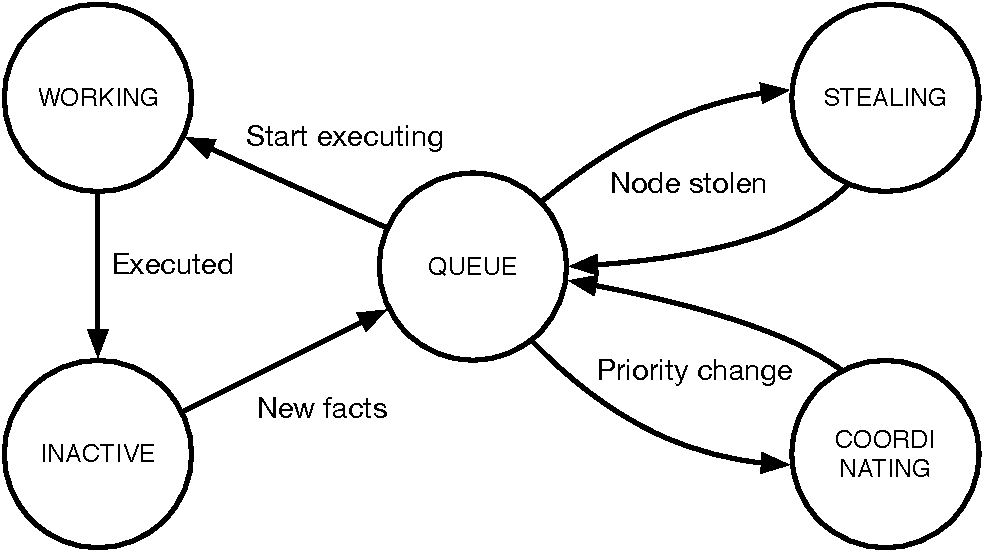
\includegraphics[width=0.55\textwidth]{figures/implementation/node_states.pdf}
   \caption{Node state machine extended with the new \textbf{coordinating}
   state.}
   \label{fig:implementation:node_states}
\end{figure}

\subsection{Coordination Instructions}\label{section:coordination:coord_instrs}

Coordination facts are implemented as API calls to the virtual machine which
implement the appropriate operations. Sensing facts read information about the
state of the virtual machine while action facts lock and update the appropriate
underlying data structures such as the node data structure or the thread's
queues.

When a thread $T_1$ performs coordination operations to a node owned by a thread
$T_2$, it needs to synchronize with $T_2$ and for that the \emph{State Lock} in
the target node needs to be acquired. Optionally, we may need to also lock the
queues of the thread $T_2$ if the priority is being updated or the queues of
thread $T_1$, if the node is moving to thread $T_1$. Note that both the standard
queue and priority queue have separate locks in order to allow concurrent
manipulation of the two data structures.

For the coordination facts \code{set-priority} and \code{add-priority}, when
multiple operations are directed to the same node during a single node
execution, we coalesce the multiple operations into a single operation.  As an
example, if a node derives two \code{set-priority} facts that change the
priority of node \code{@1} to \code{1} and \code{2}, the virtual machine
coalesces the two instructions into a single \code{set-priority} that is applied
with value \code{2} (the higher priority) after all the candidate rules of the
node are executed. The reason for this optimization is that nodes may run for
some number of steps during the lifetime of the program, therefore immediately
applying each and every coordination instruction is not cost effective. We aim
to reduce the amount of locking and movement of nodes inside the queues due to
priority updates.


\section{Coordinating SSSP}
Now that we have presented the coordination facts for LM, we are now in a
position to use them in the SSSP program presented before.  The coordinated
version of the SSSP~(Fig.~\ref{code:shortest_path_program_coord}) uses the
coordination fact \texttt{set-priority} (line 14) and a global program directive
to order priorities in ascending order (line 5).

When run with one thread, the algorithm behaves like Dijkstra's shortest path
algorithm~\cite{Dijkstra}. When using multiple threads, each thread will pick
the shortest distance from their subset of nodes.  While this does not yield the
optimal program with relation to 1 thread, it allows for parallel execution and
locally avoids unnecessary work. The result scales well and it is close to
Dijkstra's algorithm.

\begin{figure}[ht]
\begin{Verbatim}[numbers=left,xleftmargin=7mm,commandchars=\\\{\}]
type route edge(node, node, int).
type linear shortest(node, int, list int).
type linear relax(node, int, list int).

\underline{priority @order asc}.

shortest(A, +00, []).
relax(@1, 0, [@1]).

shortest(A, D1, P1), D1 > D2, relax(A, D2, P2)
   -o shortest(A, D2, P2),
      \{B, W | !edge(A, B, W) |
         relax(B, D2 + W, P2 ++ [B]),
         \underline{set-priority(B, float(D2 + W))}\}.

shortest(A, D1, P1), D1 <= D2, relax(A, D2, P2)
   -o shortest(A, D1, P1).
\end{Verbatim}
   \caption{Shortest Path Program coordinated with \texttt{set-priority}.}
   \label{code:shortest_path_program_coord}
\end{figure}

The most interesting property of the SSSP program presented in
Fig.~\ref{code:shortest_path_program_coord} is that it remains provably correct,
although it applies rules using smarter ordering and the code remains
declarative. Since the proof of correctness considers that, eventually, the
shortest path is computed at all nodes of the graph, the use of
\texttt{set-priority} does not change this at all.


\section{Applications}

To further understand how coordination facts work, we present other programs that
take advantage of them.

\subsection{Belief Propagation}

Randomized and approximation algorithms can obtain significant benefits from
coordination directives because although the final program results will not be
exact, they follow important statistical properties and can be computed faster.
An examples of such programs is PageRank~\cite{Lubachevsky:1986:CAA:4904.4801}
and Loopy Belief Propagation~\cite{Gonzalez+al:aistats09paraml}, which is the
focus of this section.

Loopy Belief Propagation (LBP) is an approximate inference algorithm used in
graphical models with cycles~\cite{Murphy99loopybelief}. In its essence, LBP is
a sum-product message passing algorithm where nodes exchange messages with their
immediate neighbors and apply some computations to the messages received.

LBP is an algorithm that maps very well to the graph-based model of LM. The
original algorithm computes the belief of all nodes for several iterations with
synchronization between iterations. However, it is possible to avoid the
synchronization step, if we take advantage of the fact that LBP will converge
even when using an asynchronous approach. So, instead of computing the belief
iteratively, we keep track of all messages sent/received (and overwrite them
when we receive a new one) and recompute the belief asynchronously.
Figure~\ref{fig:coordination:bp} shows the communication patterns for our
application and Fig.~\ref{code:coordination:bp} presents the LM code for the
implementation.

\begin{figure}[h]
   \begin{center}
      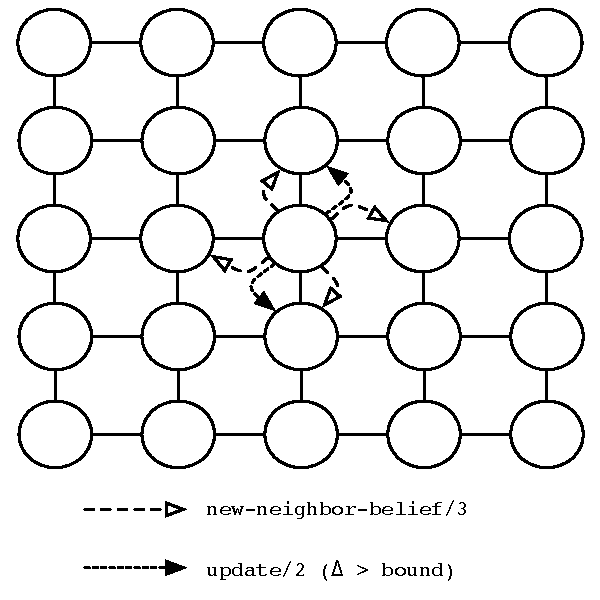
\includegraphics[width=0.3\textwidth]{figures/bp/bp.pdf}
   \end{center}
\caption{LBP: communication patterns}
\label{fig:coordination:bp}
\end{figure}

\begin{figure}[h!]
   \begin{Verbatim}[numbers=left, fontsize=\scriptsize]
neighbor-belief(A, B, Belief),
new-neighbor-belief(A, B, NewBelief)
   -o neighbor-belief(A, B, NewBelief).

check-residual(A, Residual, B),
Residual > bound
   -o update(B).
check-residual(A, _, _) -o 1.

// update belief to be sent to one neighbor
update-messages(A, NewBelief),
!edge(A, B),
neighbor-belief-old(A, B, OldIn),
sent-neighbor-belief(A, B, OldOut),
Cavity = normalize(divide(NewBelief, OldIn)),
Convolved = normalize(convolve(global-potential, Cavity)),
OutMessage = damp(Convolved, OldOut, damping)
   -o Residual = residual(OutMessage, OldOut),
      check-residual(A, Residual, B),
      update-messages(A, NewBelief),
      new-neighbor-belief(B, A, OutMessage),
      sent-neighbor-belief(A, B, OutMessage).

update-messages(A, NewBelief) -o 1.

// if we have two update functions, just run one of them
update(A), update(A) -o update(A).

// make a copy of neighbors beliefs in order to add them up
update(A),
!potential(A, Potential),
belief(A, MyBelief)
   -o [custom addfloats Potential => Belief | B, Belief |
         neighbor-belief(A, B, Belief) |
         neighbor-belief-old(A, B, Belief), neighbor-belief(A, B, Belief) |
         Normalized = normalizestruct(Belief),
         update-messages(A, Normalized), belief(A, Normalized)].
\end{Verbatim}
\caption{LM code for the Loopy Belief Propagation problem.}
\label{code:coordination:bp}
\end{figure}

Belief values are arrays of floats and are represented by \texttt{belief/2}
facts. The first rule (lines 1-3) updates a given neighbor belief whenever a new
belief value is received. This is the highest priority rule since we want to
update the neighbor beliefs before doing anything else. In order to store the
belief values of the neighbor nodes, we use \texttt{neighbor-belief/3} facts,
where the second argument is the neighbor address and the third argument is the
belief value.

The last two rules (lines 26-37) update the belief value of a node. An
\texttt{update/1} fact starts the process. The first rule (lines 27) simply
consumes redundant \texttt{update/1} facts and the second rule (lines 30-37)
performs the belief update by aggregating all the neighbor belief values. The
aggregate in lines 33-37 also derives copies of the neighbors beliefs that need
to be consumed in order to compute the belief value that is going to be sent to
the target neighbor. The aggregate uses a custom accumulator that takes two
arrays and adds the floating point numbers at each index of the array.  The rule
in lines 10-22 iterates through the neighbor belief values and sends new belief
values by performing the appropriate computations on the new belief value of the
current node and on the belief value sent previously.  Once the facts
\texttt{neighbor-belief-old} are fully consumed, the rule in line 24 is fired in
order to consume \texttt{update-messages}.

For each neighbor update, we also check in lines 5-8 if the change in belief
values is greater than \texttt{bound} (a program constant) and then force the
neighbor nodes to update their belief values by deriving \texttt{update(B)}.
This allows neighbor nodes to use updated neighbor values and recompute their
own belief values using better information. The computation of belief values
will then start to converge to their true belief values, independently of the
node scheduling used. However, if we prioritize nodes that receive new neighbor
belief values with a larger \texttt{Residual} then we will converge faster.
Figure~\ref{code:coordination:improved_bp} shows the fourth rule modified with
\texttt{add-priority} in order to increase to priority of neighbor nodes when
the source node has large changes in its belief value.

\begin{figure}[h!]
\begin{Verbatim}[numbers=left,commandchars=\\\{\},fontsize=\scriptsize]
// update belief to be sent to one neighbor
update-messages(A, NewBelief),
!edge(A, B),
neighbor-belief-old(A, B, OldIn),
sent-neighbor-belief(A, B, OldOut),
Cavity = normalize(divide(NewBelief, OldIn)),
Convolved = normalize(convolve(global-potential, Cavity)),
OutMessage = damp(Convolved, OldOut, damping)
   -o Residual = residual(OutMessage, OldOut),
      \underline{add-priority(B, Residual)},
      check-residual(A, Residual, B),
      update-messages(A, NewBelief),
      new-neighbor-belief(B, A, OutMessage),
      sent-neighbor-belief(A, B, OutMessage).
\end{Verbatim}
\caption{Updating the BP program to use priorities.}
\label{code:coordination:improved_bp}
\end{figure}


\section{Related Work}\label{sec:coordination:related}

As mentioned in Section~\ref{sec:background:coordination}, Linda~\cite{linda}
and Delirium~\cite{Delirium} are two programming languages that support
coordination. When compared to LM, Linda and Delirium are limited in the sense
that the programmer can only coordinate the scheduling of processing units,
while placement of data is left to the implementation. LM differs from those
languages because coordination acts on data instead of processing units.
Coordination facts as used in this chapter raise the abstraction by considering
data and algorithmic aspects of the program instead of focusing on how
processing units are used. Furthermore, LM is both a coordination language and a
computation language and the distinction between the two components is small.

There are also several programming models also support some kind of coordination
primitives that allow explicit scheduling and load balancing of work between
available processing units but are not considered proper programming languages.

The Galois~\cite{Pingali:2011:TPA:1993316.1993501} programming model implements
autonomous scheduling by default, where activities may be rolled back in case of
conflict. However, it is possible to employ a concrete scheduling strategy for
coordinating parallel execution in order to improve execution and avoid
conflicts.  First, there is \emph{compile-time coordination}, where the
scheduling ordered is computed during compilation and is pre-defined before the
program is executed. Secondly, there is \emph{runtime coordination}, where the
order of activities is computed during execution. The execution of the algorithm
proceeds in rounds: first, a set of non-conflicting activities is computed and
then executed by applying the operator; conflicting activities are postponed to
the next round. The third and last scheduling strategy is \emph{just-in-time
coordination} where the order of activities is defined by the underlying data
structure where the operator is applied (for instance, computing on a graph
may depend on its topology).

In the context of the Galois model, Nguyen et al.~\cite{nguyen11} expanded the
concept of runtime coordination with the introduction of a flexible approach to specify
scheduling policies for Galois programs. This approach was motivated by the fact
that some algorithms can be executed faster if computations use better
scheduling strategies. The scheduling language specifies 3 main scheduler types:
FIFO (First-In First-Out), LIFO (Last-In First-Out) and
OrderedByMetric (order activities by some metric). These schedulers can
be composed and synthesized without requiring users to write complex concurrent
code.

Elixir~\cite{Prountzos:2012:ESS:2384616.2384644} is a domain specific language
that builds on top of the Galois and allows easy specification of scheduling
strategies.  The main idea behind Elixir is that the user should be able to
specify how operator application is scheduled and the framework will compile
this high level specification to low level code using the provided scheduling
specification. One of the motivating examples is the Single Source Shortest Path
program that can be specified using multiple scheduling specifications,
generating different well-known shortest path algorithms such as the
Dijkstra or Bellman-Ford algorithm. Unlike the work of Nguyen et
all.~\cite{nguyen11}, Elixir does not allow graph mutations.

Halide~\cite{Ragan-Kelley:2013:HLC:2491956.2462176} is a language and compiler
for image processing pipelines with the goal of optimizing parallelism, locality
and re-computation. Halide decouples the algorithm definition from its execution
strategy, allowing the compiler to find which execution strategy may be the best
for optimizing for locality and parallelism. The language allows the programmer
to specify the scheduling strategy, allowing the programmer to decide the order
of computations, what intermediate results need to be stored, how to split the
data among processing units and how to use vectorization and the well-known
sliding window mechanism. However, the compiler is able to use stochastic search
to find good schedules for Halide pipelines. Notably, experimental results
indicate that automatic search sometimes leads to better execution than
hand-written code.

In contrast to the previous systems, LM stands alone in making coordination
(both scheduling and partitioning) a first-class programming construct and
semantically equivalent to computation. Furthermore, LM distinguishes itself by
supporting data-driven dynamic coordination, particularly for irregular data
structures. Elixir and Galois do not support coordination for data partitioning,
and, in Elixir, the coordination specification is separated from computation,
limiting the programmability of coordination. Compared to LM, Halide is
targeted for regular applications and therefore only supports compile time
coordination.

\section{Chapter Summary}

In this chapter, we presented the set of coordination facts, a new declarative
mechanism for coordinating declarative parallel programs. Coordination facts are
implemented as sensing and action facts and allow the programmer to write
derivation rules that change how the runtime system schedules computation and
partitions the data in the parallel system, thus improving the executing time.
In terms of programming language design, our coordination mechanisms are unique
in the sense that they are treated like regular computation, which allows for
complex run-time coordination policies that are declarative and is part of the
main program's logic.
